\documentclass{article}
\usepackage{graphicx}
\usepackage{hyperref}
\usepackage{float}
\begin{document}

\section{Dataset Information}\label{dataset-information}

\textbf{Dataset Chosen:}
 APOGEE2 from SDSS\\
\textbf{Objective:}
Identifying Young Stars and Differentiating them from Red Giants?\\
% =========================================
% =========================================
% =========================================
\section{Exploratory Data Analysis} On doing EDA we find various trends, the
following are the Observations.\\
% =========================================
\subsection{Data Density and Galactic Coordinates}
\begin{figure}[H]
   \centering
   \label{fig:1}
   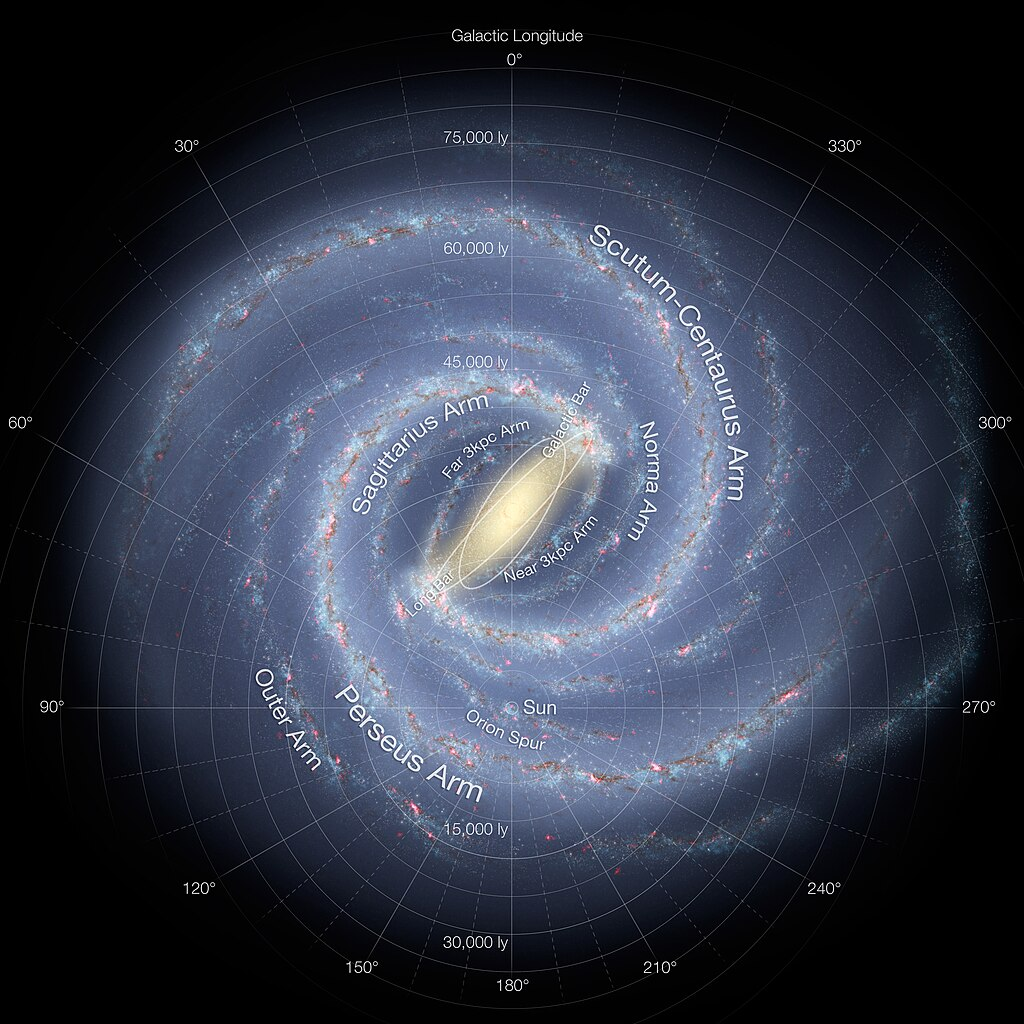
\includegraphics[width=\textwidth]{Images/GalacticCoordinates.jpg}
   \caption{Galactic Coordinate System}
\end{figure}

\paragraph{}
The \hyperref[fig:1]{Artist's depiction} Above of the Milky Way Galaxy showing the origin and orientation of galactic longitude. The galactic longitude (l) runs from the Sun upwards in the image through the center of the galaxy. The galactic latitude (b) is perpendicular to the image (i.e. coming out of the image) and also centered on the Sun.

\paragraph{}
From a the \hyperref[fig:2]{APOGEE Targetting Field Map} and \hyperref[fig:3]{Density plot} of the data points we can see that the data is slighly biased as we physically cannot observe the stars on the opposite side of our galaxy. However, the stars we can observe are well recorded. with only a few peaks in the interesting regions like the Magellanic Clouds.

\begin{figure}[H]
   \centering
   \label{fig:2}
   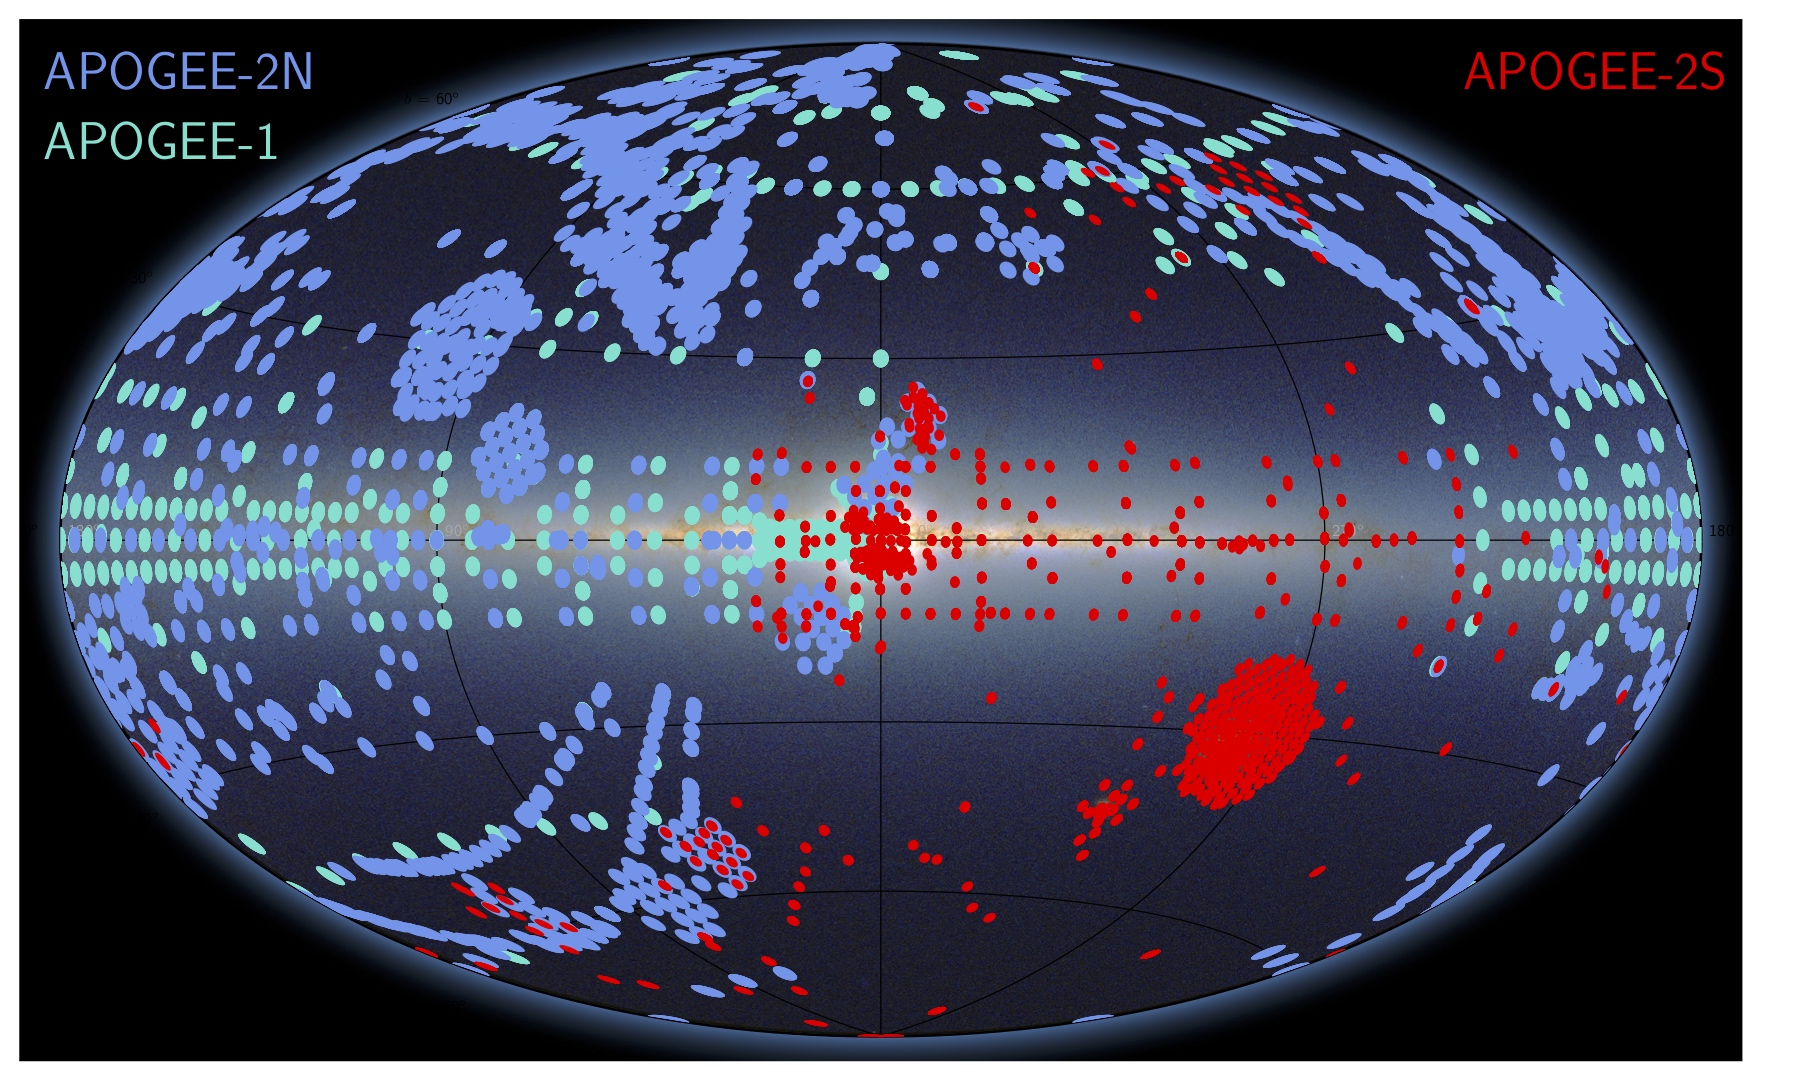
\includegraphics[width=\textwidth]{Images/ApogeeCoverage.jpg}
   \caption{DR17 APOGEE field map where the fields are color-coded by the APOGEE sub-survey. APOGEE-1 in cyan, APOGEE-2N in blue, and APOGEE-2S in red. Figure by C. Hayes. Background image from 2MASS.}
\end{figure}
\begin{figure}[H]
    \centering
    \label{fig:3}
    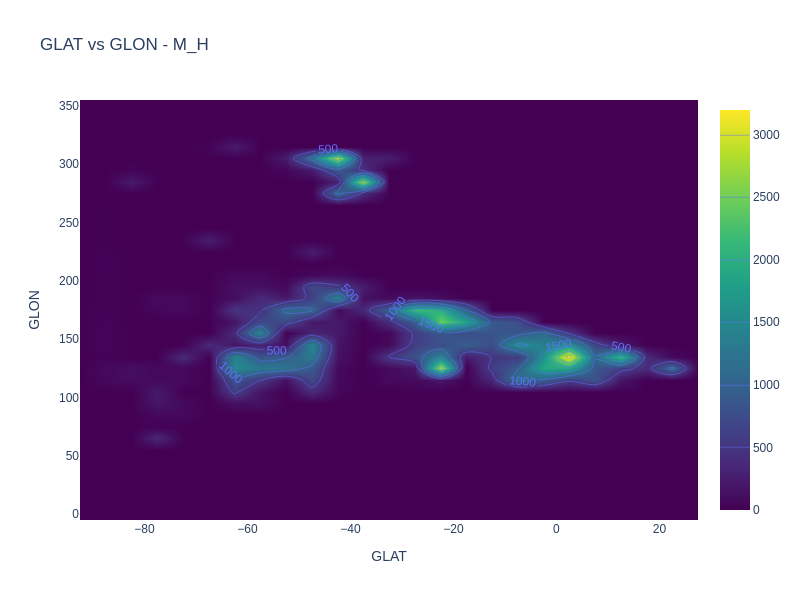
\includegraphics[width=\textwidth]{Images/GLAT vs GLON - Density.png}
    \caption{Density Plot}
\end{figure}

% =========================================
\subsection{HR Diagram}
\begin{figure}[H]
    \centering
    \label{fig:4}
    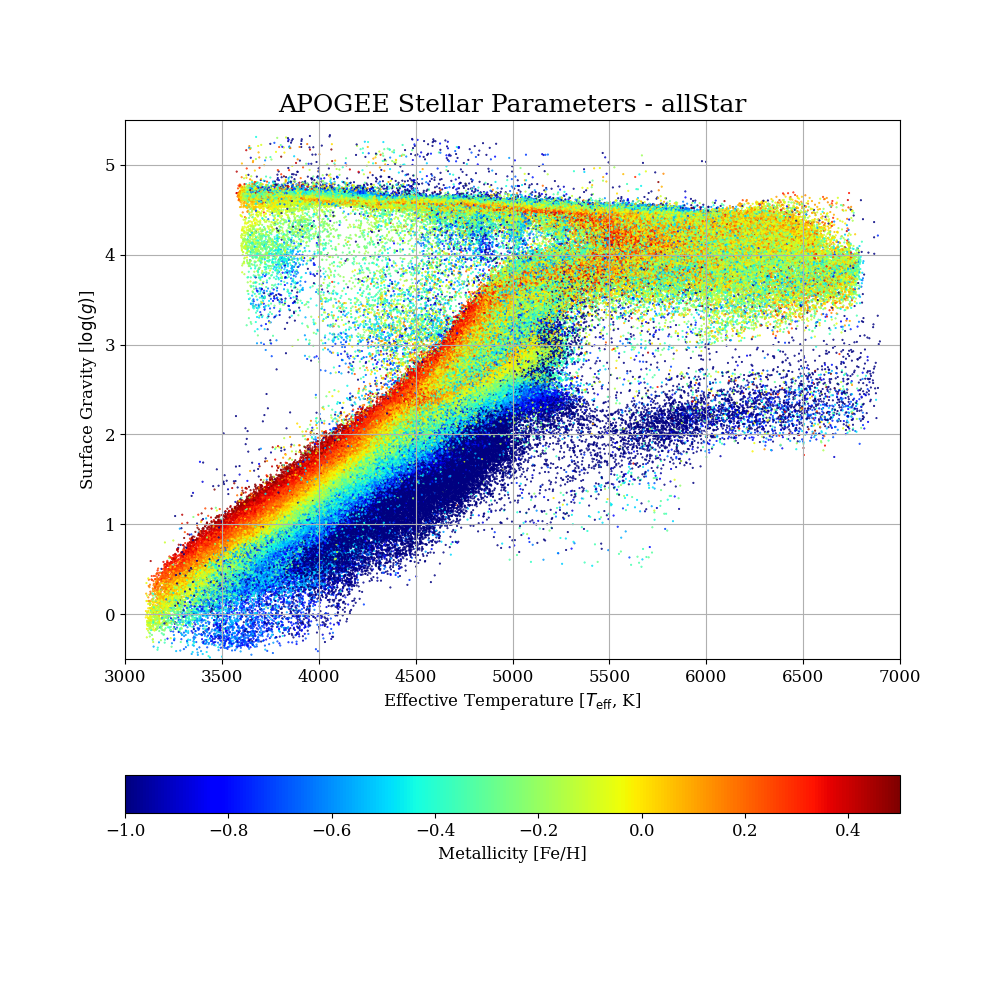
\includegraphics[width=\textwidth]{Images/APOGEEStellarParameters-allStar.png}
    \caption{HR - Diagram}
\end{figure}
From a \hyperref[fig:4]{scatterplot} between  Effective Temperature at Surface \(T_{eff}\) and the Surface Gravity \(log( g)\) we can see that:
\begin{itemize}
  \item the Relationship is mostly linear upto \(T_{eff} < 5000K\) and \(log(g) < 3\), this is known as the main sequence of stars, which is most of the lifetime of the star. Any given star moves from a lower Metallicity to a Higher Metallicity as it grows Older.

  \item The star moves above \(T_{eff} > 5000K\) and \(log(g) > 3\) when its dying, converting to various types of Dead Stars such as Red Giants, Red Supergiants, White Dwarfs, Neutron Stars and Black holes depending on a mixture of various variables.
\end{itemize}
% =========================================
\subsection{Star Formation Regions}
\begin{figure}[H]
    \centering
    \label{fig:5}
    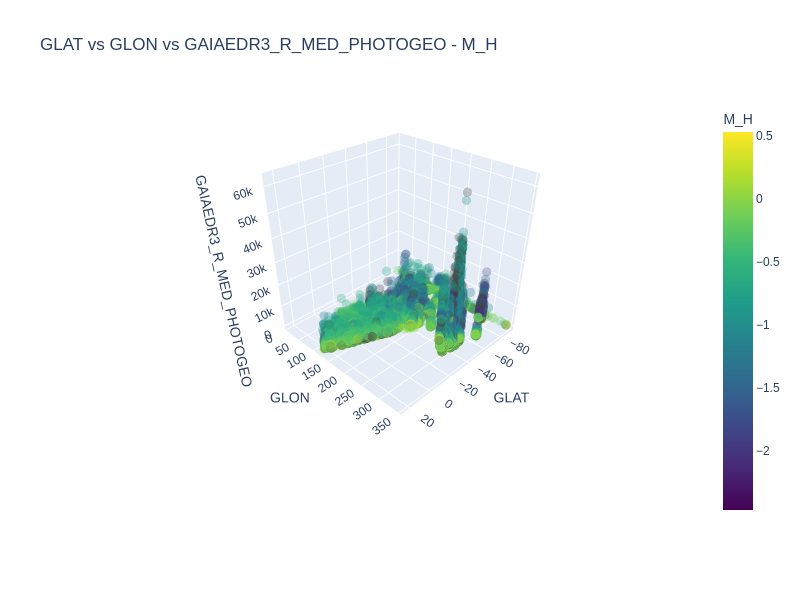
\includegraphics[width=\textwidth]{Images/GLAT vs GLON vs Distance - M_H.png}
    \caption{GLAT vs GLON vs Distance Colored by M_H}
\end{figure}
\paragraph{}
In the above \hyperref[fig:3]{Scatterplot} we can Identify the various regions with a high star formation rate. They can be identified by the clumps of datapoints which are a deep blue.
\paragraph{}
The Deep-Blue Signifies a Low Metallicity which means that the particular star is Young.
% =========================================
\section{Feature Selection}\label{feature-selection}

Techniques Applied: - Correlation Matrix

% =========================================
\subsection{Correlation Matrix}
We create the Covariance Matrix Heatmap and Remove Highly Correlated Features with \( | r |  > 0.85 \):\\

\begin{figure}[H]
    \centering
    \label{fig:6}
    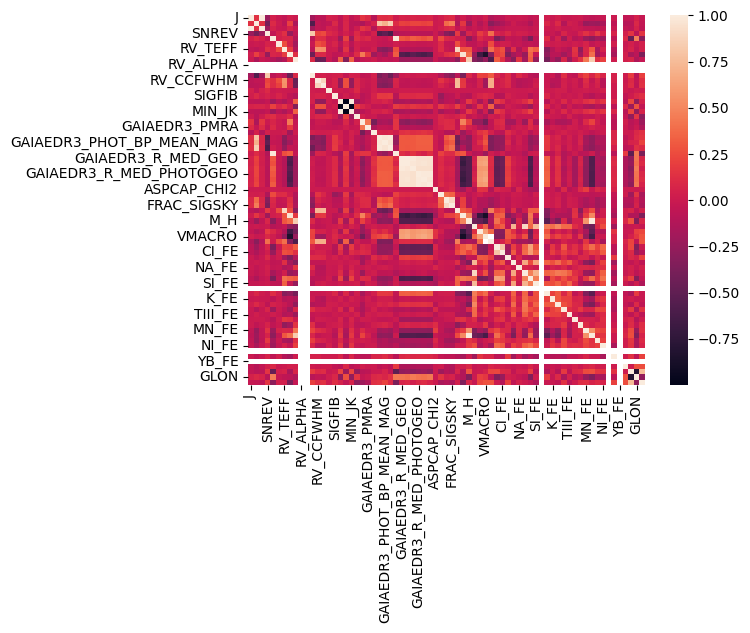
\includegraphics[width=\textwidth]{Images/CorrelationMatrixBetweenNumerical1.png}
    \caption{HR - Diagram}
\end{figure}


After Dropping we get the following columns left:
\paragraph{}
{[}`J', `H', `K',
`SNREV', `VHELIO\_AVG', `VSCATTER', `RV\_TEFF', `RV\_LOGG', `RV\_FEH',
`RV\_ALPHA', `RV\_CARB', `RV\_CHI2', `RV\_CCFWHM', `RV\_AUTOFWHM',
`MEANFIB', `SIGFIB', `MIN\_H', `MAX\_H', `MIN\_JK', `MAX\_JK',
`GAIAEDR3\_PARALLAX', `GAIAEDR3\_PMRA', `GAIAEDR3\_PMDEC',
`GAIAEDR3\_PHOT\_G\_MEAN\_MAG', `GAIAEDR3\_PHOT\_BP\_MEAN\_MAG',
`GAIAEDR3\_PHOT\_RP\_MEAN\_MAG', `GAIAEDR3\_DR2\_RADIAL\_VELOCITY',
`GAIAEDR3\_R\_MED\_GEO', `GAIAEDR3\_R\_LO\_GEO', `GAIAEDR3\_R\_HI\_GEO',
`GAIAEDR3\_R\_MED\_PHOTOGEO', `GAIAEDR3\_R\_LO\_PHOTOGEO',
`GAIAEDR3\_R\_HI\_PHOTOGEO', `ASPCAP\_CHI2', `FRAC\_BADPIX',
`FRAC\_LOWSNR', `FRAC\_SIGSKY', `TEFF', `LOGG', `M\_H', `ALPHA\_M',
`VMICRO', `VMACRO', `VSINI', `C\_FE', `CI\_FE', `N\_FE', `O\_FE',
`NA\_FE', `MG\_FE', `AL\_FE', `SI\_FE', `P\_FE', `S\_FE', `K\_FE',
`CA\_FE', `TI\_FE', `TIII\_FE', `V\_FE', `CR\_FE', `MN\_FE', `FE\_H',
`CO\_FE', `NI\_FE', `CU\_FE', `CE\_FE', `YB\_FE', `RA', `DEC', `GLON',
`GLAT'{]}
% =========================================



\end{document}
